%%%%%%%%%%%%%%%%%%%%%%%%%%%%%%%%%%%%%%%%%%%%%%
%                insertmeeting
% 1) Title (something creative & funny?)
% 2) Date (MM/DD/YYYY)
% 3) Location (ex. Hagerty High School)
% 4) People/Committees Present 
% 5) Picture 
% 6) Start Time & Stop Time (ex. 12:30AM to 4:30PM)
%%%%%%%%%%%%%%%%%%%%%%%%%%%%%%%%%%%%%%%%%%%%%%
\insertmeeting 
	{The Return of Scoopie} 
	{01/15/22} 
	{Hagerty High School}
	{Annika, Clayton, Falon, James, Jensen, Nathan, Ritam, Rose, Samantha, Lilly}
	{Images/RobotPics/robot.jpg}
	{2:30 - 4:30}
	
\hhscommittee{General}
\noindent\hfil\rule{\textwidth}{.4pt}\hfil
\subsubsection*{Goals}
\begin{itemize}
    \item Evaluate the changes we made on robot and their effectiveness
    \item Assess how we can improve Scoopie
    \item Review the strategies other teams were doing
  

\end{itemize} 

\noindent\hfil\rule{\textwidth}{.4pt}\hfil

\subsubsection*{Accomplishments}
TITLE: RETURN OF SCOOPIE
The Mechromancers had the fourth meet of the season January 15th at Melbourne, Florida. Our team ranked in 1st place! While only our drive team was able to go to the meet the hype was still there as our members joined the livestream to cheer them on. Again for this meet one of our huge issues was a lack of driver practice.  With this meet  suddenly coming a week after the last, we only had enough time to make some adjustments to our intake and were unable to address the improvements to the autonomous that we wanted to make. However the new adjustments to the intake were enough to make driver practice vital and that put us in a significant disadvantage compared to meet 3, where we had lots of driver practice.
- Work on new intake design
- Finish updates on the autonomous 
- Practice lots with the new intake design before leagues
This meet was a huge eye opener about all the improvements we need to make before leagues. After taking the new intake design to the meet we realized that the robot not being able to pick up both blocks and balls put us at a huge disadvantage because having to stop to choose the correct cargo ate away at all of the time that was saved by the robot's speed. Also due to the quick turn around between meet 3 and meet 4 we were unable to finish the autonomous improvements that we wanted to make after the last meet. We hope that with the new autonomous system we will be able to start getting blocks in auto during the leagues. Overall this meet was a huge success for Scoopie and the team. We learned lots from our mistakes and feel we have enough time before leagues to make all the adjustments and improvements to Scoopie that we want to make! 

 

\begin{figure}[ht]
\centering
\begin{minipage}[b]{.48\textwidth}
  \centering
  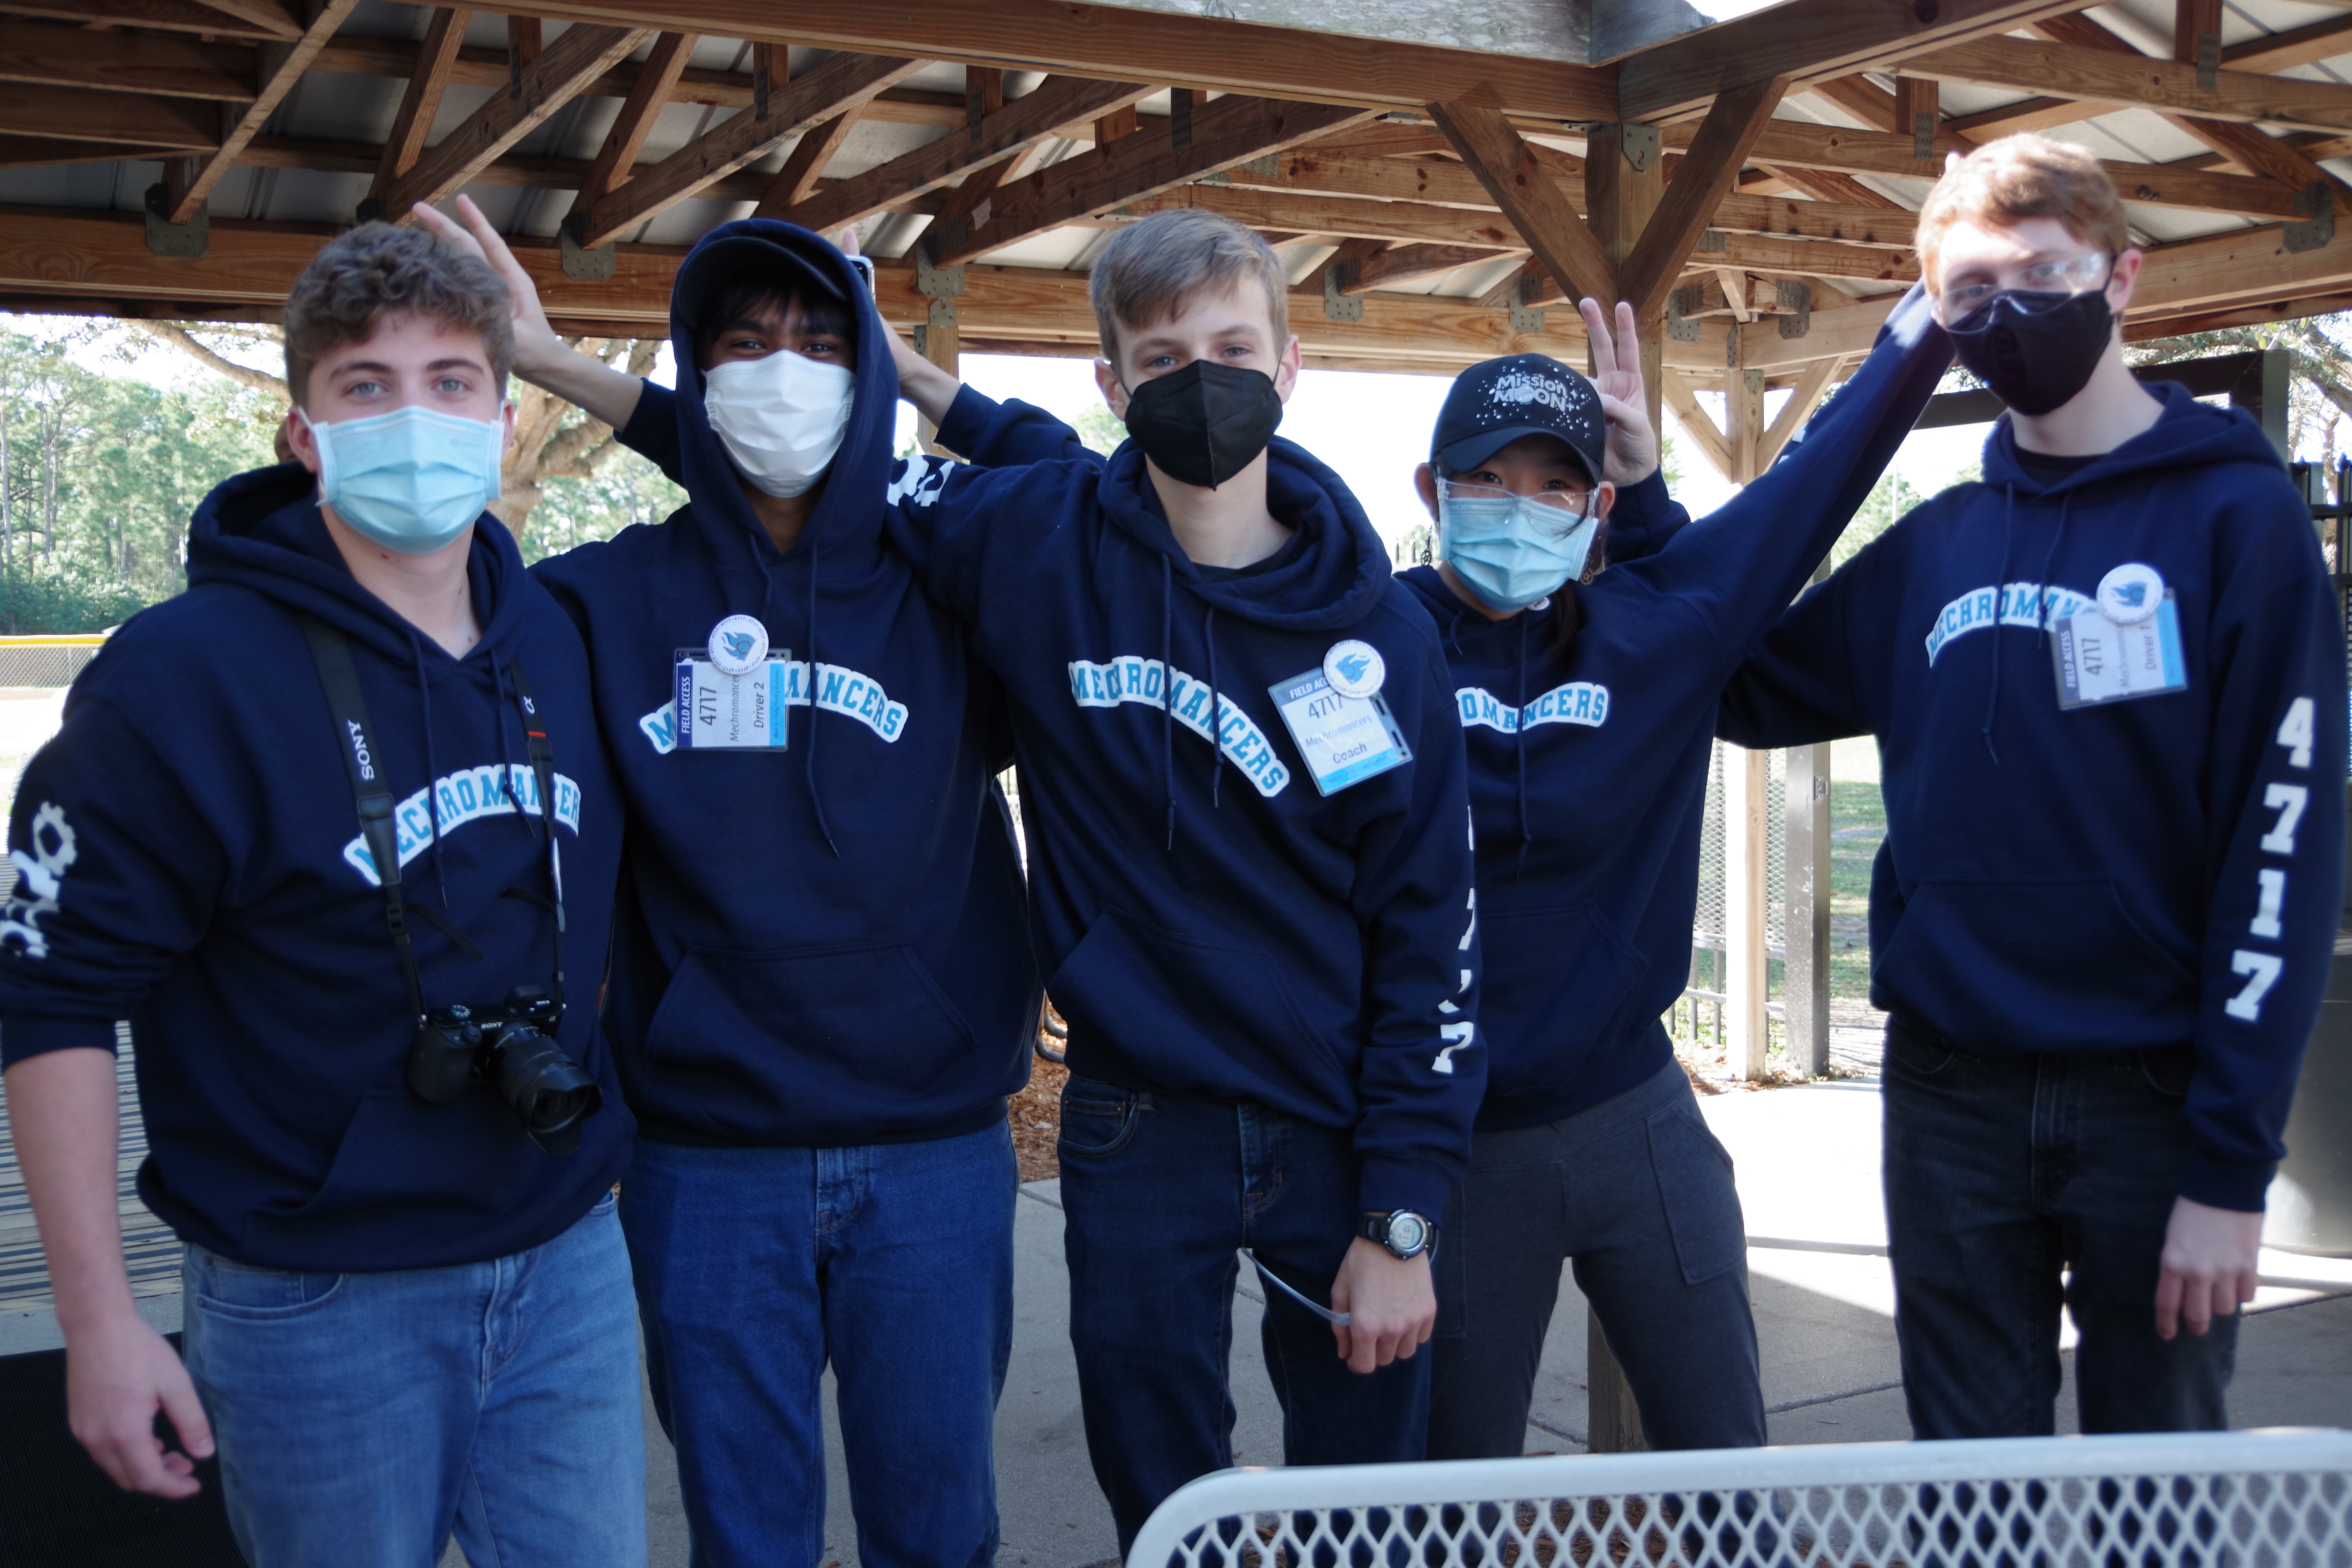
\includegraphics[width=0.95\textwidth]{Meetings/January/01-15-22/1-15-22_Team_Figure1 - Nathan Forrer.JPG}
  \caption{4717 at Meet 4}
  \label{fig:011522_1}
\end{minipage}%
\hfill%
\begin{minipage}[b]{.48\textwidth}
  \centering
  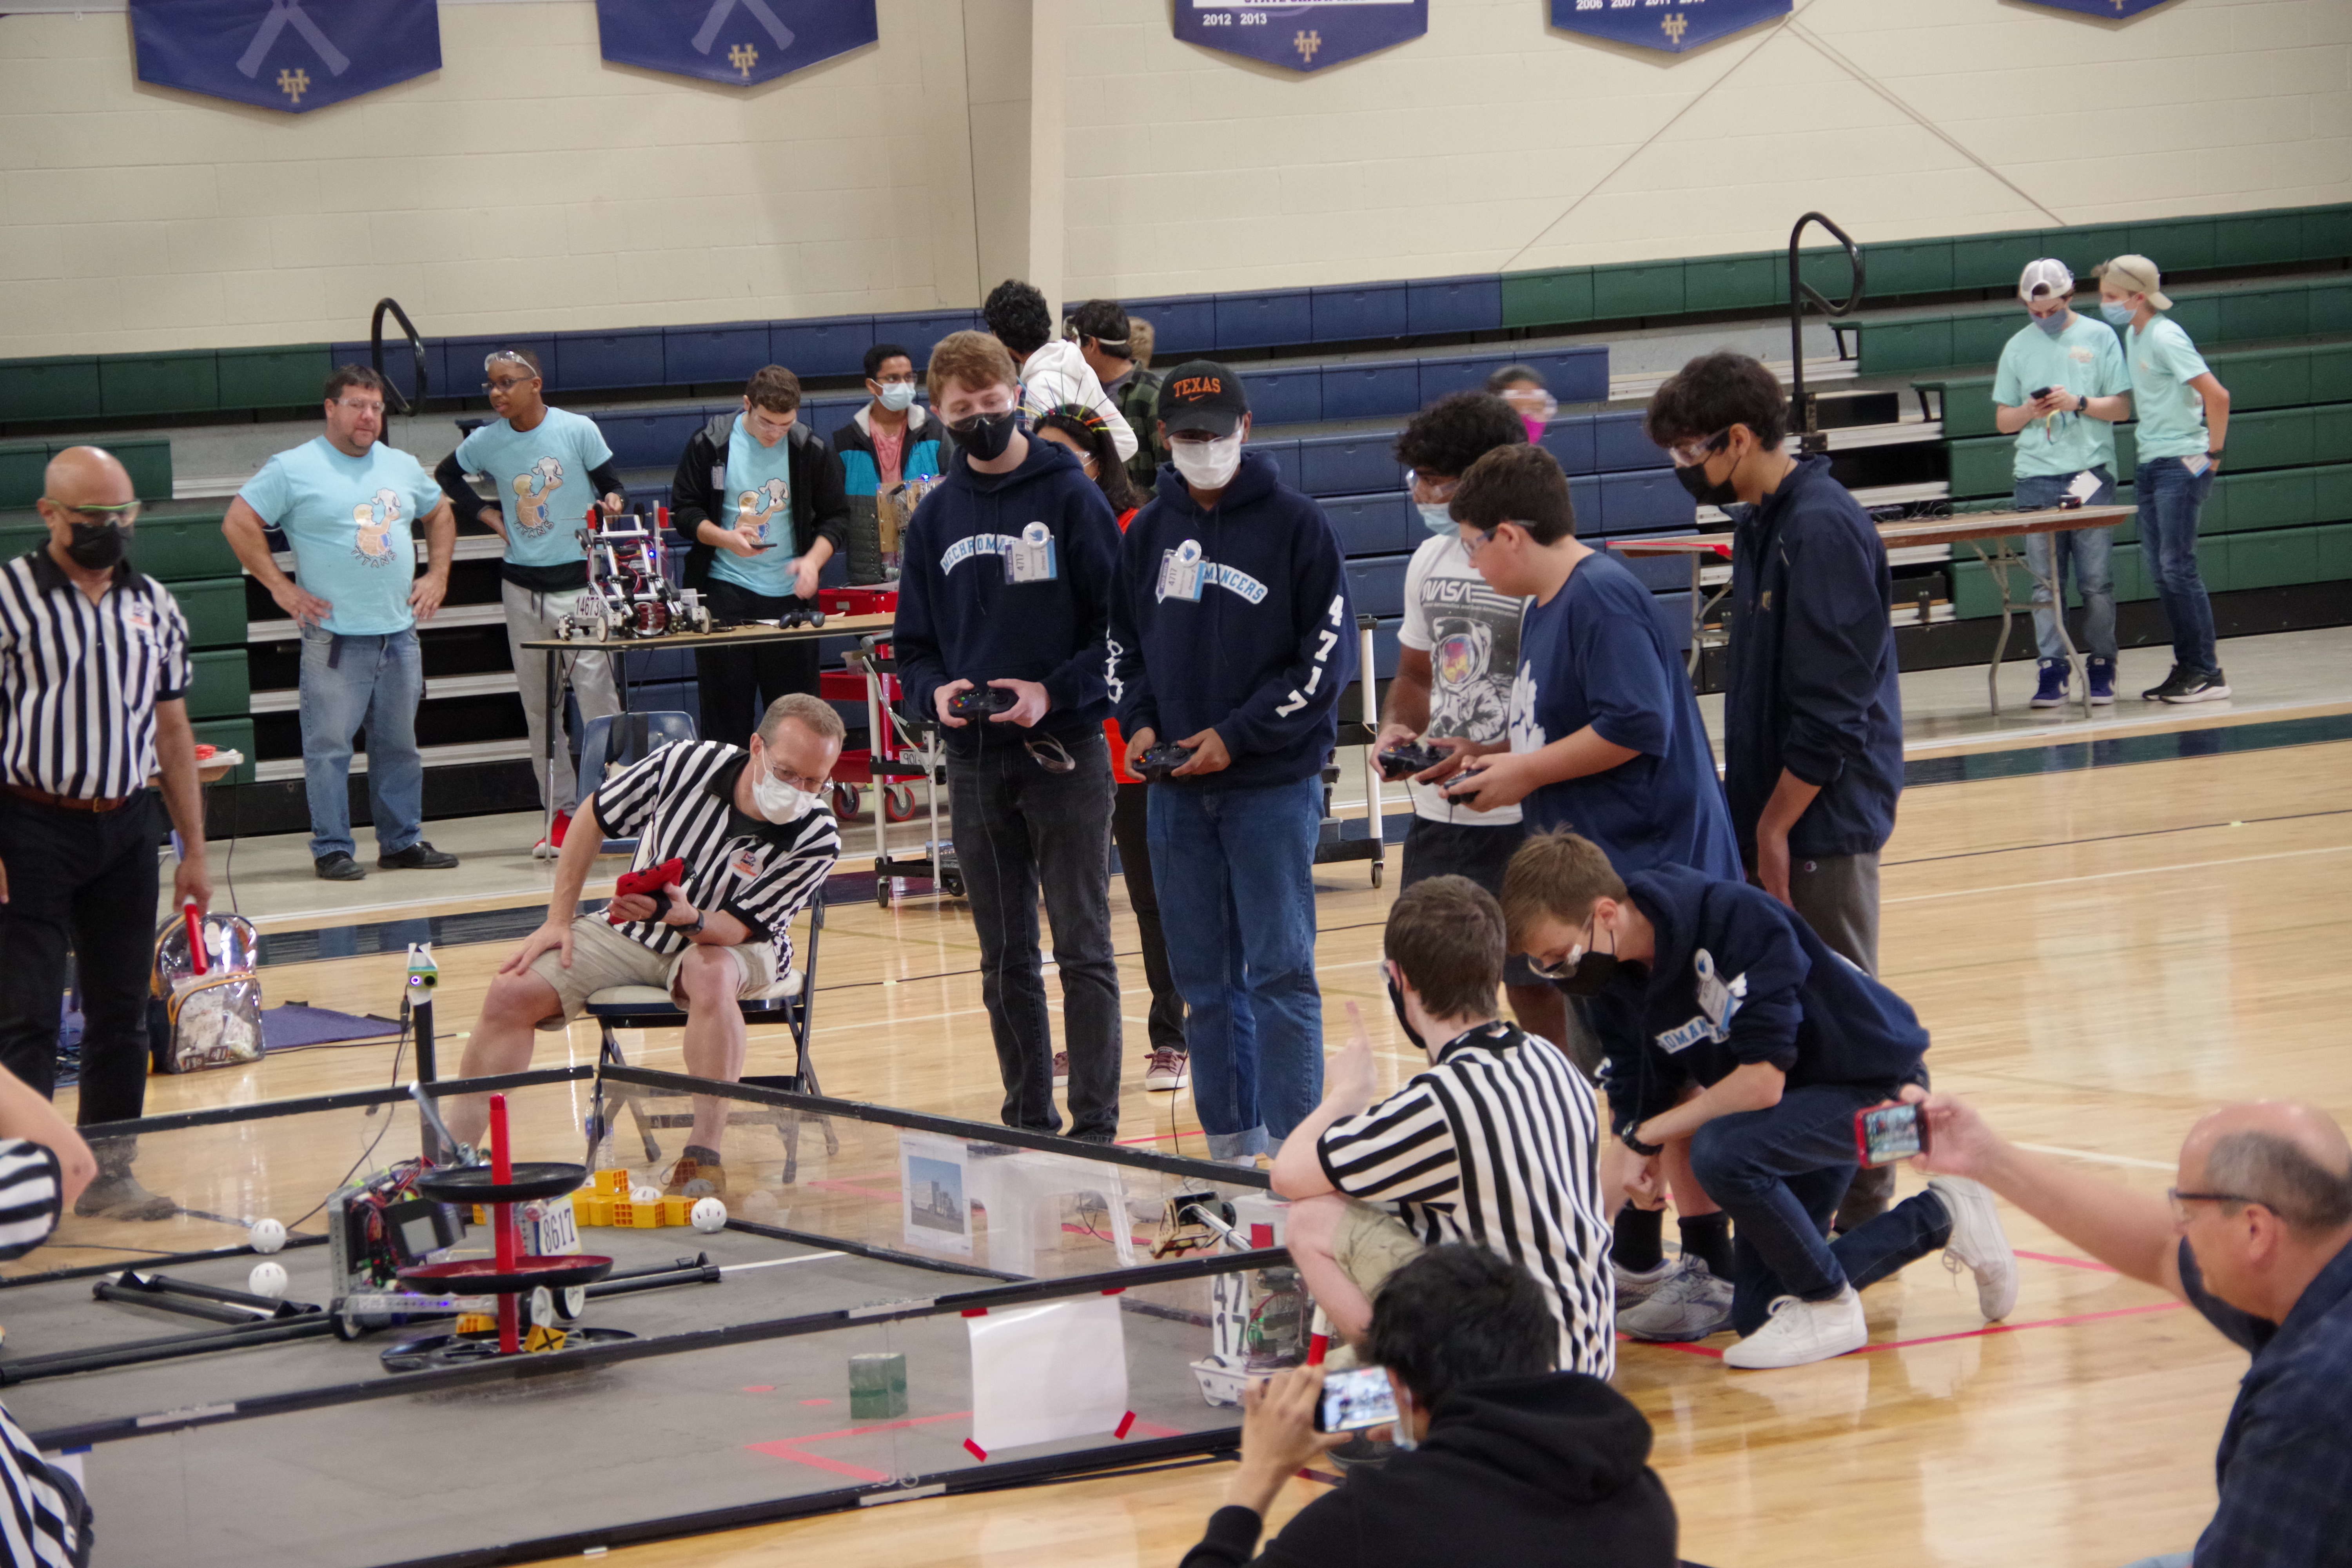
\includegraphics[width=0.95\textwidth]{Meetings/January/01-15-22/1-15-22_Team_Figure2 - Nathan Forrer.JPG}
  \caption{Intense competition}
  \label{fig:011522_2}
\end{minipage}
\end{figure}

\begin{figure}[htp]
\centering
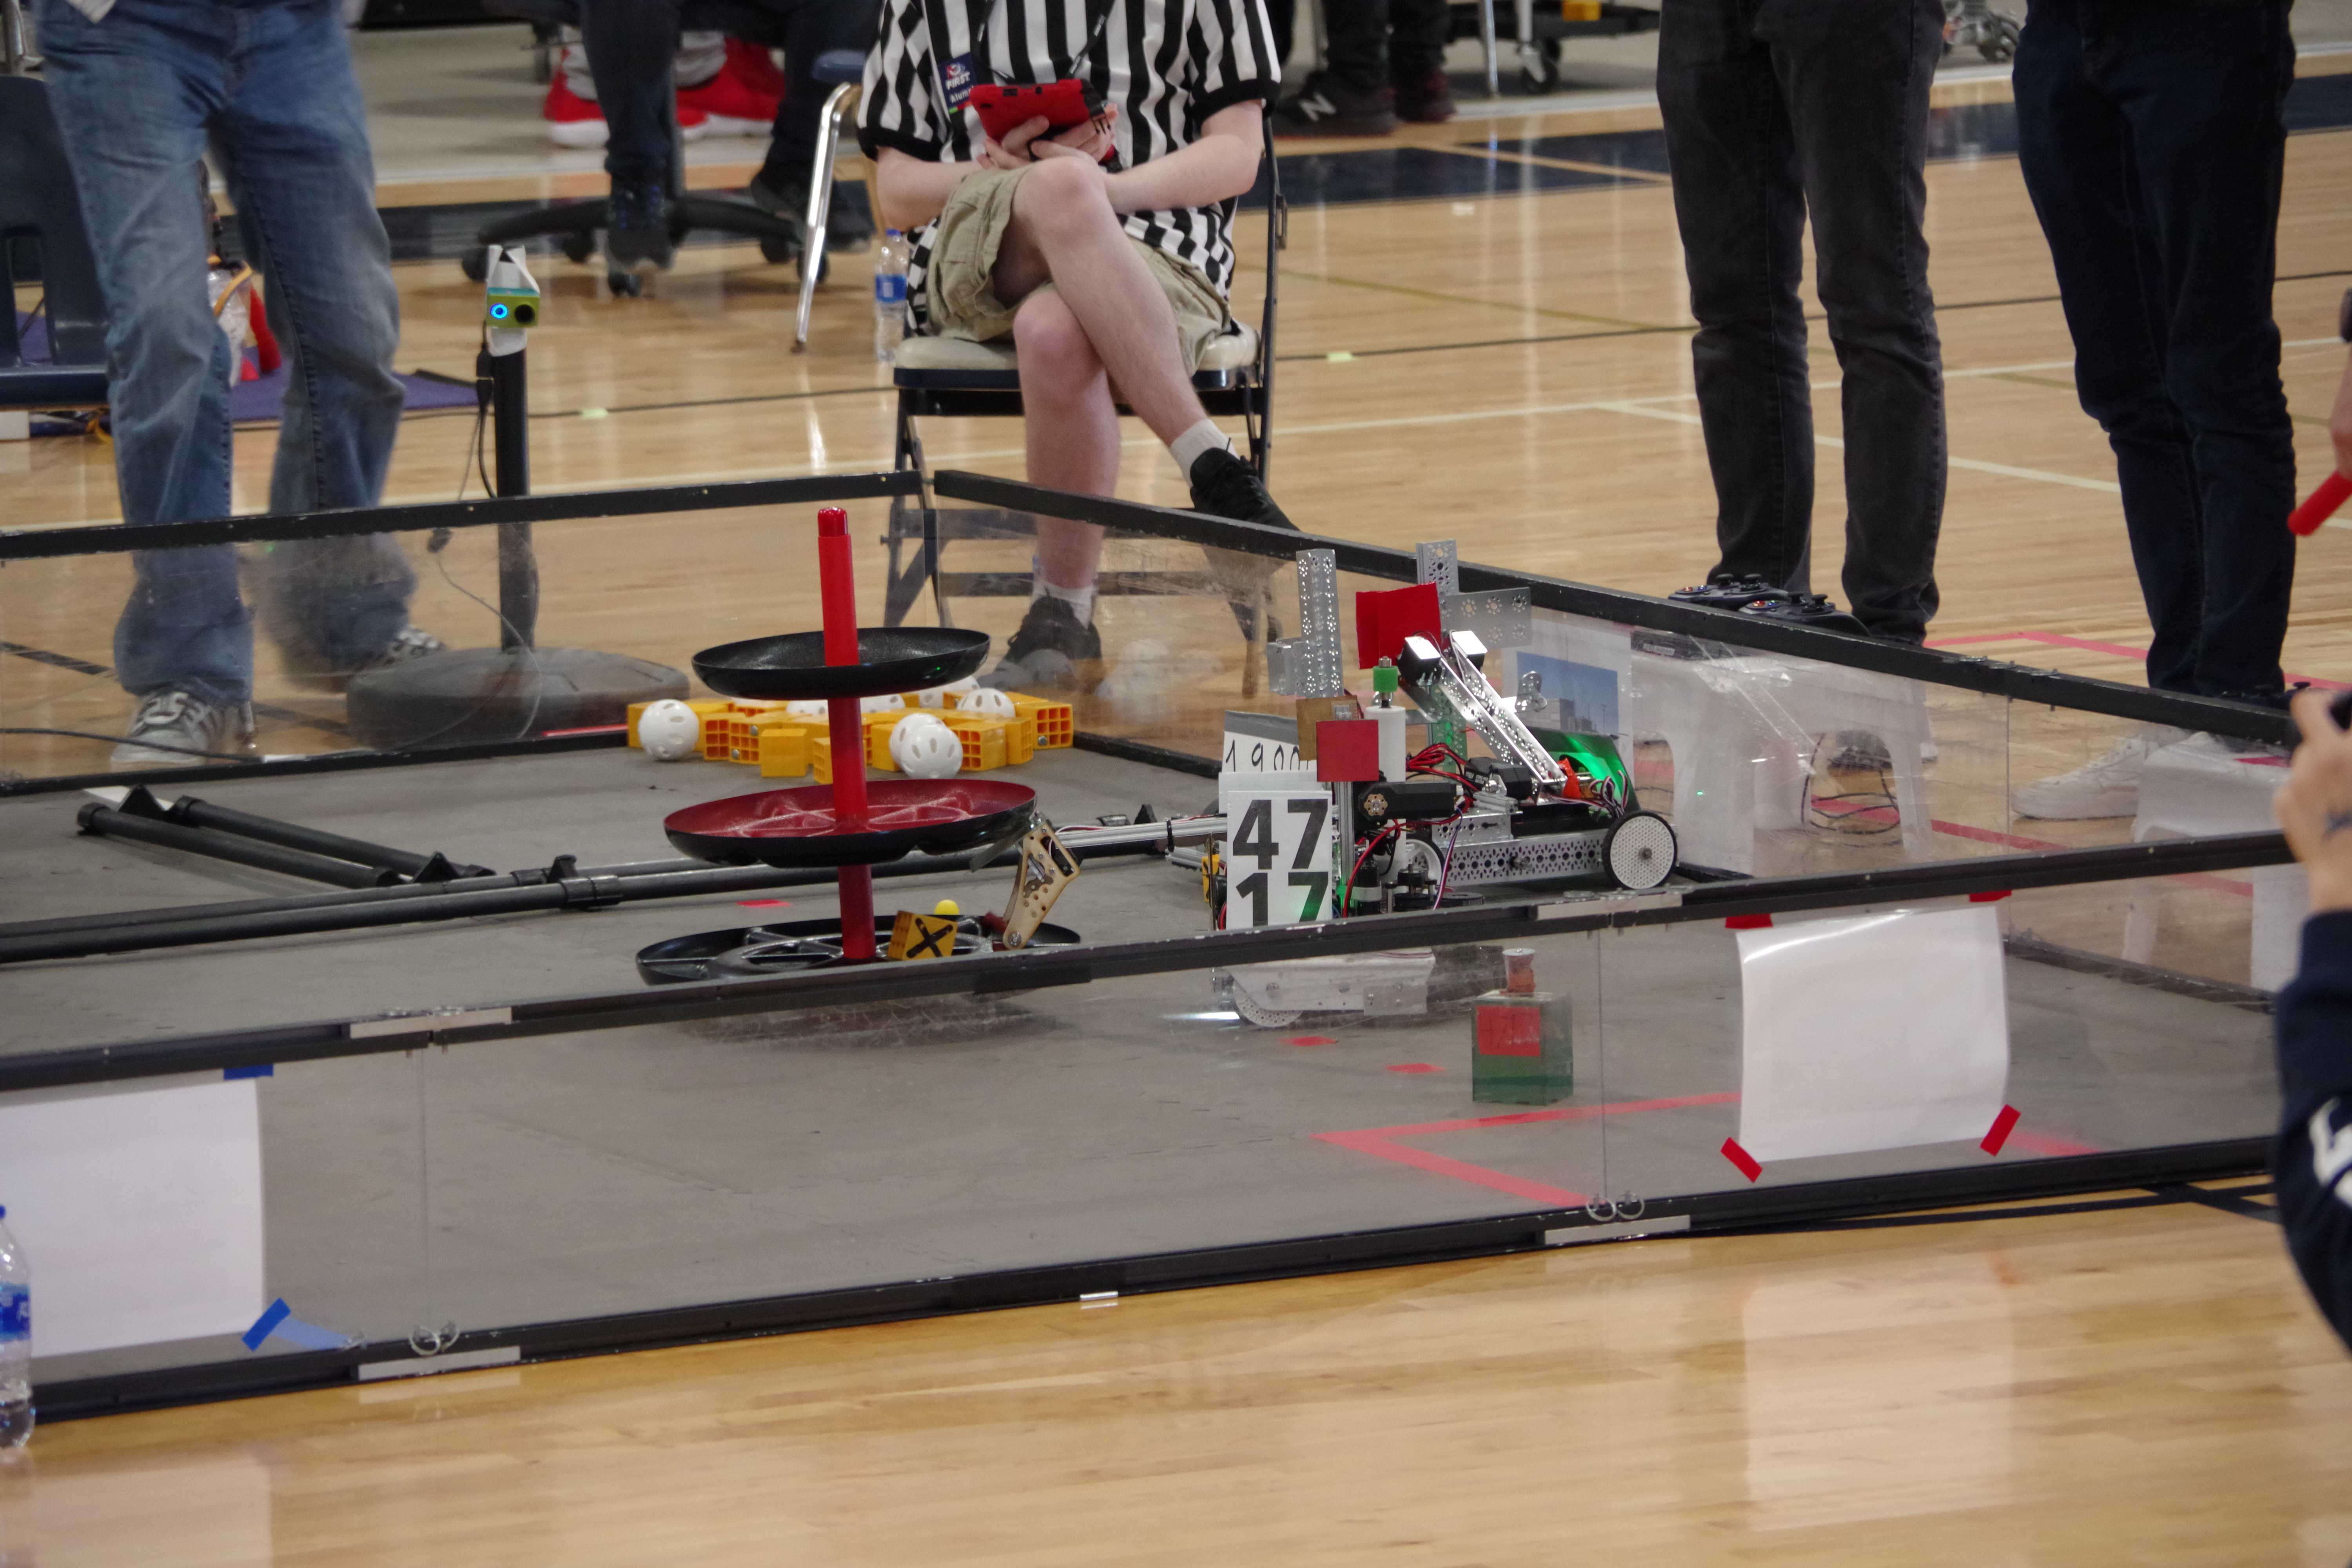
\includegraphics[width=0.95\textwidth, angle=0]{Meetings/January/01-15-22/1-15-22_Team_Figure3 - Nathan Forrer.JPG}
\caption{Scoopie in Action}
\label{fig:011522_3}
\end{figure}

\whatsnext{
\begin{itemize}
    \item redesign intake to be able to intake balls
    \item add cycles to autonomous
    \item do more driver practice before leagues
\end{itemize} 
}

